\documentclass[11pt,a4paper]{article}
\usepackage[margin=20mm]{geometry}
\usepackage{fontspec,amsmath,amssymb,tikz,enumitem,xcolor,fancyhdr}
\usetikzlibrary{arrows.meta,calc}
\setmainfont{FreeSerif}[Scale=1.04]
\setsansfont{FreeSerif}
\XeTeXlinebreaklocale "th_TH"
\XeTeXlinebreakskip=0pt plus 1pt
\setlength{\parindent}{0pt}
\setlength{\parskip}{5pt}
\pagestyle{fancy}\fancyhf{}\lhead{\small PHYSICS OLYMPIAD / CAMP 1}\rhead{\small Problems 001--010}\cfoot{\thepage}
\newcommand{\prob}[2]{\par\vspace{12pt}{\large\bfseries #1}\hfill{\small\color{gray} #2}\par\vspace{4pt}}
\begin{document}
{\Huge\bfseries Physics Olympiad}\par
{\Large คลังโจทย์ฟิสิกส์ สอวน. ค่าย 1}\par
{\small โจทย์ข้อ 1--10}
\hrule
\prob{MEC-0001}{ต้นฉบับข้อ 1}
ถังน้ำทรงกระบอกรัศมี $R$ ความสูง $H$ ใส่น้ำจนเต็ม เมื่อตั้งถัง จากนั้นจึงจับเอียงทำมุม $\theta$ กับแนวดิ่ง จะเหลือน้ำในถังเป็นปริมาตรเท่าใด
\begin{center}
\begin{tikzpicture}[scale=.83,>=Latex]
\draw[thick] (-.4,0)--(5,0) node[right]{พื้นระดับ};
\draw[thick] (1,0)--(2.2,3.2) (2.3,0)--(3.5,3.2);
\draw[thick] (1.65,0) ellipse (.65 and .16);
\draw[thick] (2.85,3.2) ellipse (.65 and .16);
\draw[blue!60!black,thick] (1.12,.34)--(2.55,.34);
\draw[dashed] (1,0)--(1,3.4);
\draw[->] (1,1.05) arc[start angle=90,end angle=69,radius=1.05];
\node at (1.35,1.55) {$\theta$};
\node at (3.38,1.55) {$H$};\node at (3.8,3.55) {$R$};
\draw[->] (.05,2.65)--(.05,2.05) node[below] {$g$};
\end{tikzpicture}
\end{center}
\prob{MEC-0002}{ต้นฉบับข้อ 2}
ชายคนหนึ่งสูง 2 เมตร ยืนอยู่ที่ชายฝั่งทะเล มองผิวน้ำทะเลไกลออกไปจนสุดขอบฟ้า ถ้าโลกเป็นทรงกลมรัศมี 6370 กิโลเมตร จงประมาณว่าสุดขอบฟ้าที่ชายคนนั้นเห็นอยู่ไกลจากที่เขายืนกี่กิโลเมตร
\prob{MEC-0003}{ต้นฉบับข้อ 3}
บ้านกับโรงเรียนอยู่ห่างกันเป็นระยะทาง $L$ รถของเราเคลื่อนที่ด้วยความเร็วคงที่ $v$ ในการวิ่งจากบ้านไปโรงเรียน กำหนดในที่นี้ว่าอัตราการเผาผลาญน้ำมันเชื้อเพลิงของรถคือ $R$ ซึ่ง $R=Av^2+B$, $A$ กับ $B$ เป็นค่าคงที่สำหรับรถ จงหาค่าความเร็ว $v_m$ ของรถที่จะทำให้หมดเปลืองเชื้อเพลิงน้อยที่สุดในการวิ่งจากบ้านไปโรงเรียน ตอบในรูปของ $A$ กับ $B$
\begin{center}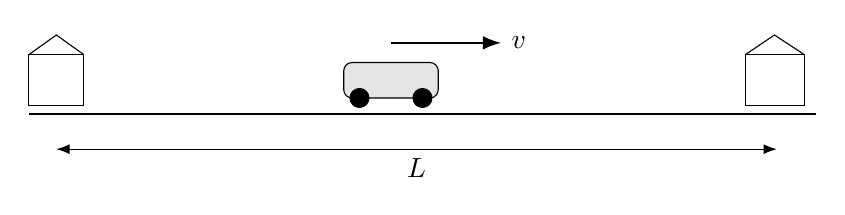
\begin{tikzpicture}[>=Latex]
\draw[thick] (0,0)--(10,0);
\draw (0,.1) rectangle (.7,.75);\draw (.0,.75)--(.35,1)--(.7,.75);
\draw (9.1,.1) rectangle (9.85,.75);\draw (9.1,.75)--(9.47,1)--(9.85,.75);
\draw[rounded corners=3pt,fill=gray!20] (4,.2) rectangle (5.2,.65);
\draw[fill=black] (4.2,.2) circle (.12) (5,.2) circle (.12);
\draw[->,thick] (4.6,.9)--(6,.9) node[right]{$v$};
\draw[<->] (.35,-.45)--(9.5,-.45) node[midway,below]{$L$};
\end{tikzpicture}\end{center}
\par\noindent\fcolorbox{gray!50}{gray!5}{\begin{minipage}{.88\linewidth}\small
คำแนะนำจากต้นฉบับ: ฟังก์ชัน $y(x)=ax+\dfrac{b}{x}$ และจุดต่ำสุด $(x_m,y_m)$ สัมพันธ์กับสมการ $ax_m^2-y_mx_m+b=0$ (ภาพกราฟคำแนะนำในต้นฉบับยังไม่ได้วาดใหม่)\end{minipage}}
\clearpage\prob{MEC-0004}{ต้นฉบับข้อ 4}
อัตราเร็ว $v$ ของคลื่นผิวน้ำความตึงผิว $\gamma$ ความหนาแน่น $\rho$ เมื่อความยาวคลื่นเป็น $\lambda$ เป็นไปตามสมการ
\[v^2=\frac{g}{2\pi}\lambda+\frac{2\pi\gamma}{\rho}\frac{1}{\lambda}\]
ซึ่งบ่งว่า $v_m$ เป็นอัตราเร็วที่ต่ำสุด (ต่ำกว่าไม่มี) ที่ความยาวคลื่น $\lambda_m$
\begin{enumerate}[label=4.\arabic*.,leftmargin=1.2cm]
\item จงแก้สมการ Quadratic Equation ใน $\lambda$ เพื่อหาค่า $v_m$ ในเทอมของ $\gamma,\rho$ และ $g$ ทั้งนี้ โดยอาศัยเงื่อนไขที่ว่าที่จุดต่ำสุดนั้น รากของสมการเป็น $\lambda_1=\lambda_2=\lambda_m$
\item ต่อไปใช้ $\gamma=75$ กรัมต่อวินาที$^2$, $\rho=1$ กรัมต่อซม.$^3$ และ $g=980$ ซม.ต่อวินาที$^2$ แล้วหาค่าของ $v_m$ ในหน่วย cm\,s$^{-1}$ ออกมา
\end{enumerate}
\begin{center}\begin{tikzpicture}[>=Latex,xscale=1.0,yscale=.65]
\draw[->] (0,0)--(6.2,0) node[right]{$\lambda$};\draw[->] (0,0)--(0,4.5) node[above]{$v^2$};
\draw[thick,domain=.35:5.8,samples=80] plot (\x,{.45*\x+1.3/\x});
\draw[dashed] (1.7,0) node[below]{$\lambda_m$}--(1.7,1.53)--(0,1.53) node[left]{$v_m^2$};
\fill (1.7,1.53) circle (2pt);
\end{tikzpicture}\end{center}
\prob{MEC-0005}{ต้นฉบับข้อ 5}
คาบการแกว่งของลูกตุ้มนาฬิกา $T$ เป็นไปตามสมการ $T=2\pi\sqrt{l/g}$ โดยที่ $l$ คือความยาวของเชือกที่แขวนลูกตุ้ม ถ้าเราทำการทดลองวัดคาบ $T$ ที่ความยาวเชือก $l$ ต่างๆ แล้วนำข้อมูลมาเขียนกราฟระหว่าง $T^2$ กับ $l$ ความชันของเส้นกราฟที่ได้ควรจะเท่ากับปริมาณต่อไปนี้
\begin{enumerate}[label=\arabic*.,itemsep=0pt]
\item $\dfrac{l}{T^2}$ \item $\dfrac{2\pi}{\sqrt g}$ \item $\dfrac{4\pi^2}{g}$ \item $\dfrac{T}{\sqrt l}$
\end{enumerate}


\prob{MEC-0006}{ต้นฉบับข้อ 6}
(USO รอบที่ 1 2555) ความถี่ $f$ ของมวล $m$ ติดสปริง เป็นไปตามสมการ
\[ f=\frac{1}{2\pi}\sqrt{\frac{k}{m}} \]
เมื่อ $k$ คือค่าคงตัวของสปริง ถ้าเราทำการทดลองวัดค่า $f$ เมื่อเปลี่ยนมวล $m$ ไปเรื่อยๆ เราควรเขียนกราฟระหว่างปริมาณใดต่อไปนี้ เพื่อให้ได้กราฟเป็นเส้นตรง
\begin{enumerate}[label=\arabic*.,itemsep=0pt]
\item $f^2$ กับ $\dfrac{1}{m}$
\item $f$ กับ $m$
\item $f$ กับ $\sqrt{m}$
\item $\dfrac{1}{f}$ กับ $m$
\end{enumerate}
\prob{MEC-0007}{ต้นฉบับข้อ 7}
(USO รอบที่ 1 2555) แรง $A$ และแรง $B$ กระทำต่อวัตถุที่ตำแหน่ง $X$ ด้วยขนาดและทิศทางดังแสดงด้วยลูกศร ดังรูป ถ้าต้องการให้วัตถุอยู่ในสมดุล จะต้องออกแรง $F$ กระทำต่อวัตถุที่ตำแหน่ง $X$ ด้วย รูปสามเหลี่ยมในข้อใดต่อไปนี้แสดงความสัมพันธ์ระหว่างแรงทั้งสามได้ถูกต้อง
\begin{center}
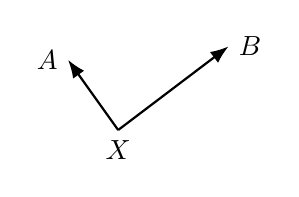
\begin{tikzpicture}[>=Latex,scale=.85,thick]
\coordinate (X) at (0,0);
\draw[->] (X)--(-.75,1.05) node[left] {$A$};
\draw[->] (X)--(1.65,1.25) node[right] {$B$};
\node[below] at (X) {$X$};
\end{tikzpicture}
\end{center}
\begin{center}
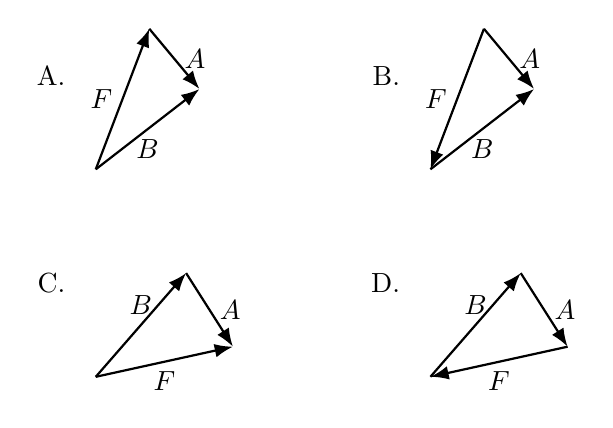
\begin{tikzpicture}[>=Latex,thick,scale=.85]
% each choice is a vector triangle; arrows distinguish directions
\begin{scope}[shift={(0,0)}]
\node[left] at (-.3,1.4) {A.};
\coordinate (P) at (0,0);\coordinate (Q) at (.8,2.1);\coordinate (R) at (1.55,1.2);
\draw[->] (P)--(Q) node[midway,left] {$F$};\draw[->] (Q)--(R) node[midway,right] {$A$};\draw[->] (P)--(R) node[midway,below] {$B$};
\end{scope}
\begin{scope}[shift={(5,0)}]
\node[left] at (-.3,1.4) {B.};
\coordinate (P) at (0,0);\coordinate (Q) at (.8,2.1);\coordinate (R) at (1.55,1.2);
\draw[<-] (P)--(Q) node[midway,left] {$F$};\draw[->] (Q)--(R) node[midway,right] {$A$};\draw[->] (P)--(R) node[midway,below] {$B$};
\end{scope}
\begin{scope}[shift={(0,-3.1)}]
\node[left] at (-.3,1.4) {C.};
\coordinate (P) at (0,0);\coordinate (Q) at (1.35,1.55);\coordinate (R) at (2.05,.45);
\draw[->] (P)--(Q) node[midway,above] {$B$};\draw[->] (Q)--(R) node[midway,right] {$A$};\draw[->] (P)--(R) node[midway,below] {$F$};
\end{scope}
\begin{scope}[shift={(5,-3.1)}]
\node[left] at (-.3,1.4) {D.};
\coordinate (P) at (0,0);\coordinate (Q) at (1.35,1.55);\coordinate (R) at (2.05,.45);
\draw[->] (P)--(Q) node[midway,above] {$B$};\draw[->] (Q)--(R) node[midway,right] {$A$};\draw[<-] (P)--(R) node[midway,below] {$F$};
\end{scope}
\end{tikzpicture}
\end{center}
\prob{MEC-0008}{ต้นฉบับข้อ 8}
(สอวน ม.4 2546) จงแปลงค่าของความเร็ว $v=4$ เมตรต่อวินาทีให้อยู่ในหน่วยมิลลิเมตรต่อวินาที
\prob{MEC-0009}{ต้นฉบับข้อ 9}
(สอวน ม.5 2546) จงแปลงค่าของพลังงานจลน์ $\dfrac{1}{2}mv^2=5$ จูล ไปอยู่ในหน่วยกรัม (มิลลิเมตรต่อวินาที)$^2$
\prob{MEC-0010}{ต้นฉบับข้อ 10}
(สอวน ม.4 2547) ความชัน 1 มิลลิเมตรต่อ 1 เมตร คิดเป็น 1 นิ้วต่อกี่ฟุต
\end{document}
